% ─────────────────────────────────────────────────────────────────────────────
% CS3315 Final Project Report — NGAFID
% Aviation Engine Health Monitoring via Machine Learning
% Iván Barbosa Mejía · NPS MSCS Q3 · 2026
% Compile: make  (pdflatex → bibtex → pdflatex × 2)
% ─────────────────────────────────────────────────────────────────────────────
\documentclass[10pt]{article}

\providecommand{\StudentName}{Iván Barbosa Mejía}
\providecommand{\CourseCode}{CS3315}
\providecommand{\CourseName}{Introduction to Machine Learning \& Big Data}
\providecommand{\ProfessorName}{Prof.  Marko Orescanin}
\providecommand{\DepartmentName}{Department of Computer Science}
\providecommand{\QuarterInfo}{MSCS Q3 · 2026}
\providecommand{\ReportTitle}{Aviation Engine Health Monitoring\\via Machine Learning}
\providecommand{\ReportSubtitle}{NGAFID: Anomaly Detection \& Fault Classification on a Real Cessna-172 Fleet}
\providecommand{\OrganizationName}{Naval Postgraduate School}
\providecommand{\LocationName}{Monterey, California}
\providecommand{\SubmissionDate}{\today}

% config/config.tex

% --- encoding ---
\usepackage[utf8]{inputenc}
\usepackage[T1]{fontenc}
\usepackage[english]{babel}

% --- fonts ---
\usepackage{newpxtext}
\usepackage{newpxmath}

% --- page layout ---
\usepackage[
  letterpaper,
  margin=1in,
  headheight=14.5pt,
  includeheadfoot
]{geometry}

% --- spacing and typography ---
\usepackage{setspace}
\onehalfspacing
\usepackage{microtype}
\setlength{\parindent}{0.5in}
\setlength{\parskip}{0pt}
\usepackage{indentfirst}

% --- math and symbols ---
\usepackage{amsmath}
\let\openbox\relax
\usepackage{amsthm}

% --- graphics / tables ---
\usepackage{graphicx}
\usepackage{booktabs}
\usepackage{array}
\usepackage{longtable}
\usepackage{tabularx}
\usepackage{caption}
\usepackage{float}
\captionsetup{font=small, labelfont=bf}

% --- color / links ---
\usepackage{xcolor}
\definecolor{npsblue}{RGB}{0,51,102}
\usepackage[
  colorlinks=true,
  linkcolor=npsblue,
  citecolor=npsblue,
  urlcolor=npsblue
]{hyperref}

% --- headers / footers ---
\usepackage{fancyhdr}
\pagestyle{fancy}
\fancyhf{}
%\fancyhead[L]{\nouppercase{\leftmark}}
\fancyhead[L]{\CourseCode\ -- \ReportSubtitle}
\fancyhead[R]{\StudentName}
\fancyfoot[C]{\thepage}
\renewcommand{\headrulewidth}{0.4pt}
\renewcommand{\footrulewidth}{0pt}

% Ensure article sections populate marks nicely
\makeatletter
\renewcommand{\sectionmark}[1]{\markboth{#1}{}}
\makeatother

% --- section formatting ---
\usepackage{titlesec}
\titleformat{\section}{\large\bfseries}{\thesection.}{0.5em}{}
\titleformat{\subsection}{\normalsize\bfseries}{\thesubsection}{0.5em}{}
\titleformat{\subsubsection}{\normalsize\itshape}{\thesubsubsection}{0.5em}{}

% --- theorem environments ---
\theoremstyle{definition}
\newtheorem{definition}{Definition}[section]
\newtheorem{example}{Example}[section]
\theoremstyle{plain}
\newtheorem{theorem}{Theorem}[section]
\theoremstyle{remark}
\newtheorem*{remark}{Remark}

% --- bibliography ---
\usepackage[numbers]{natbib}

% --- code listings ---
\usepackage{listings}
\lstset{
  basicstyle=\ttfamily\small,
  breaklines=true,
  frame=single,
  numbers=left,
  numberstyle=\scriptsize,
  stepnumber=1,
  numbersep=8pt,
  showstringspaces=false,
  tabsize=4
}


% ─── extra packages for this report ──────────────────────────────────────────
\usepackage{multirow}
\usepackage{amsmath}
% newpxmath (loaded in config) already defines \Bbbk; release it so amssymb
% can load without an "already defined" clash.
\let\Bbbk\relax
\usepackage{amssymb}
\usepackage{tikz}
\usetikzlibrary{arrows.meta, positioning}
\usepackage{pgfplots}
\pgfplotsset{compat=1.18}

% ─── title page macro (reused from study notes template) ─────────────────────
\newcommand{\MakeNPSTitlePage}{%
\begin{titlepage}
    \thispagestyle{empty}
    \begin{center}
        \vspace*{0.8cm}
        {\Large\textbf{\OrganizationName}\\[0.15cm]}
        {\large \LocationName\\[1.2cm]}
        
\includegraphics[width=0.23\textwidth]{images/logo_NPS.png}\\[1.0cm]
        {\Large \DepartmentName\\[1.2cm]}
        {\huge\bfseries \ReportTitle\\[0.35cm]}
        {\Large \ReportSubtitle\\[1.1cm]}
        \begin{tabular}{rl}
            \textbf{Course:}     & \CourseCode\ --- \CourseName \\
            \textbf{Instructor:} & \ProfessorName \\
            \textbf{Student:}    & \StudentName \\
            \textbf{Quarter:}    & \QuarterInfo \\
            \textbf{Date:}       & \SubmissionDate \\
            \textbf{Code:}       & \url{https://github.com/Barbosa12/NGAFID} \\
        \end{tabular}
        \vfill
    \end{center}
\end{titlepage}
}

% ─────────────────────────────────────────────────────────────────────────────
\begin{document}

\pagenumbering{roman}
\MakeNPSTitlePage

\begin{abstract}
This report presents a machine learning study on aviation engine health monitoring
using the National General Aviation Flight Information Database (NGAFID), a
real-world dataset of 11{,}446 flights from a Cessna-172 flight school fleet
labeled with 19 fault categories and correlated with over 2{,}000 unscheduled
maintenance events. We formulate the problem as a two-stage pipeline: binary
Anomaly Detection (AD) followed by 19-class Fault Classification (FC). Multiple
classical models (Logistic Regression, SVM, XGBoost, Random Forest) are trained
on flight-level statistical feature representations and benchmarked against
deep learning models reported in the literature, including ConvTokMHSA, MMK~Net,
and the LMSD framework \cite{lmsd2025}. Our best classical system achieves
F1~=~0.703 on AD (tuned Ensemble, 224 features) and, on FC, F1~=~0.207 for a flat
classifier and F1~=~0.459 for an Oracle K\,=\,4 hierarchical ceiling, versus the
indicative DL figures of 0.799 and 0.623 respectively---figures we treat as
indicative only, since the source preprint was subsequently withdrawn by its
authors over metric-computation flaws. The analysis shows that global statistical
features are competitive for binary detection, but a sizeable gap persists on FC
because fault signatures concentrate in low-variance principal components (notably
PC9 and PC19--23), contributing less than 0.1\% of total variance and remaining
largely invisible to global statistics. The end-to-end pipeline achieves
F1~=~0.131, with fault typing (Stage~2 wrong-type errors, 20.0\% of predictions)
the dominant error source.
\end{abstract}

\tableofcontents
\clearpage

\setcounter{page}{1}
\pagenumbering{arabic}

% ─────────────────────────────────────────────────────────────────────────────
\section{Introduction}
\label{sec:intro}
% ─────────────────────────────────────────────────────────────────────────────

\subsection{Motivation}

General aviation in the United States operates under a predominantly
\textit{calendar-based} maintenance paradigm: aircraft are inspected at fixed
intervals of hours, days, or calendar cycles regardless of the actual condition
of their components. This reactive approach systematically fails to detect
emerging faults between inspection windows, creating safety risks and generating
costly unscheduled maintenance events that grounding aircraft without warning.

Modern aircraft are equipped with flight data recorders (FDR) and engine control
units (ECU) that continuously log dozens of sensor channels at 1\,Hz or higher.
This operational data, accumulated across thousands of flight hours, encodes the
health history of every critical subsystem. Machine learning offers a principled
path from raw telemetry to \textit{condition-based} maintenance: instead of
waiting for a calendar date, a model can flag anomalous flights and identify the
likely fault category from the sensor profile alone, enabling targeted
interventions before failure occurs.

\subsection{Dataset and Scope}

This project uses the \textbf{National General Aviation Flight Information
Database (NGAFID)} \cite{ngafid2021}, a publicly available benchmark comprising
over 28{,}000 real flights from a Cessna-172 fleet operated by an active flight
school. NGAFID is unique among aviation health datasets in that it provides
(i) authentic multi-sensor telemetry under real operational conditions,
(ii) fault labels derived from verified unscheduled maintenance records
spanning 36 distinct categories, and (iii) a standardized 5-fold cross-validation
split designed to prevent data leakage between flights of the same aircraft
\cite{convtok2023}.

The analysis focuses on the \textit{benchmark 2-day subset}: 11{,}446 flights
across 19 fault categories, preprocessed to fixed length via cubic spline
interpolation to 2{,}048 time steps per flight.

\subsection{Research Questions}

This report investigates two core questions:

\begin{enumerate}
    \item \textbf{Anomaly Detection (AD):} Can a classical ML classifier, trained
          on statistical features extracted from the full flight profile, reliably
          distinguish healthy flights from anomalous ones?
    \item \textbf{Fault Classification (FC):} Given that a flight is anomalous,
          can the same approach identify which of 19 fault types is responsible?
\end{enumerate}

Both tasks are then composed into a single \textbf{End-to-End (E2E) diagnosis
pipeline} that assigns one of 20 labels---\textit{healthy} or one of 19
fault types---to any incoming flight.

\subsection{Hypothesis}

We hypothesize that:

\begin{itemize}
    \item For \textbf{AD}, global statistical features (mean, standard deviation,
          slope, etc.\ over the full flight) are sufficient to characterize the
          overall health state of the aircraft, making classical models competitive
          with deep learning.
    \item For \textbf{FC}, fault signatures manifest as \textit{local micro-patterns}
          in specific temporal segments of the flight profile, contributing less
          than 0.1\% of total variance. Global statistics discard this information,
          creating a structural performance gap versus temporal deep learning models
          that operate directly on the raw time series.
\end{itemize}

\subsection{Contributions}

The main contributions of this work are:

\begin{enumerate}
    \item A systematic evaluation of five classical ML models across multiple
          feature representations (Repr.~B through Repr.~F\textsubscript{++}) on
          the NGAFID benchmark subset, with direct comparison against published
          deep learning results \cite{lmsd2025}.
    \item A feature engineering analysis that identifies cross-physical
          inter-cylinder features (CHT/EGT spreads and ratios) as the most
          informative additions beyond global per-sensor statistics.
    \item A hierarchical fault classification experiment (Oracle K\,=\,4) that
          raises the classical ceiling from F1\,=\,0.121 to F1\,=\,0.420 through
          physics-based fault grouping, closing over half the gap to the DL best
          (MMK~Net, F1\,=\,0.623) without any temporal modeling.
    \item An end-to-end error decomposition showing that 40.6\% of E2E errors
          originate in Stage~2 (wrong fault type), identifying fault classification
          as the bottleneck for future improvement.
\end{enumerate}

\subsection{Report Organization}

The remainder of this report is organized as follows.
Section~\ref{sec:dataset} describes the NGAFID dataset, sensor space, class
distribution, and key data challenges.
Section~\ref{sec:features} presents the feature engineering pipeline and the
hierarchy of representations from global statistics to temporal shape.
Section~\ref{sec:methodology} details the two-stage diagnosis pipeline, the
classical and deep learning models, and the evaluation protocol.
Section~\ref{sec:results} reports and analyzes results for AD, FC, and E2E
across all representations, with comparison to DL benchmarks.

\newpage
% ─────────────────────────────────────────────────────────────────────────────
\section{Dataset Description}
\label{sec:dataset}
% ─────────────────────────────────────────────────────────────────────────────

\subsection{NGAFID Overview}

The National General Aviation Flight Information Database (NGAFID) is a
real-world benchmark for aircraft health diagnosis research. It was collected
from a Cessna-172 fleet operated by an active flight school and correlates
23-dimensional sensor measurements with verified unscheduled maintenance records.
Table~\ref{tab:ngafid_overview} summarizes the key characteristics of the
dataset.

\begin{table}[H]
    \centering
    \caption{NGAFID dataset overview.}
    \label{tab:ngafid_overview}
    \begin{tabular}{ll}
        \toprule
        \textbf{Property} & \textbf{Value} \\
        \midrule
        Aircraft type         & Cessna-172 \\
        Operator              & Real flight school (anonymized) \\
        Total flights         & $>$28{,}000 (31{,}000 flight hours) \\
        Sensor channels       & 23 @ 1\,Hz \\
        Maintenance categories & 36 \\
        Unscheduled events    & $>$2{,}000 \\
        Preprocessing         & Forward-fill for NaN; cubic spline $\to$ 2{,}048 pts \\
        \midrule
        \multicolumn{2}{l}{\textit{Benchmark subset (2-day) — used in this work}} \\
        Total flights         & 11{,}446 \\
        Healthy flights       & 5{,}845 (51.1\%) \\
        Anomalous flights     & 5{,}601 (48.9\%) \\
        Fault classes (FC)    & 19 \\
        Cross-validation      & 5-fold stratified, physically isolated \\
        \bottomrule
    \end{tabular}
\end{table}

NGAFID provides two dataset configurations: the \textit{benchmark subset}
(19 classes, 11{,}446 flights) used for controlled evaluation, and the
\textit{overall dataset} (36 classes, 28{,}935 flights) for open-environment
assessment. This study uses the benchmark subset exclusively.

\subsection{Sensor Space}

The 23 sensor channels cover five critical aircraft subsystems.
Table~\ref{tab:sensors} lists all channels grouped by subsystem.

\begin{table}[H]
    \centering
    \caption{23-dimensional sensor space organized by subsystem.}
    \label{tab:sensors}
    \begin{tabular}{llc}
        \toprule
        \textbf{Subsystem} & \textbf{Channels} & \textbf{Count} \\
        \midrule
        Electrical   & \texttt{volt1}, \texttt{volt2}, \texttt{amp1}, \texttt{amp2} & 4 \\
        Fuel         & \texttt{FQtyL}, \texttt{FQtyR} & 2 \\
        Engine       & \texttt{E1 FFlow}, \texttt{E1 OilT}, \texttt{E1 OilP}, \texttt{E1 RPM} & 4 \\
        Cylinders (CHT) & \texttt{E1 CHT1}, \texttt{E1 CHT2}, \texttt{E1 CHT3}, \texttt{E1 CHT4} & 4 \\
        Cylinders (EGT) & \texttt{E1 EGT1}, \texttt{E1 EGT2}, \texttt{E1 EGT3}, \texttt{E1 EGT4} & 4 \\
        Flight state & \texttt{IAS}, \texttt{VSpd}, \texttt{AltMSL}, \texttt{NormAc} & 4 \\
        Environment  & \texttt{OAT} & 1 \\
        \midrule
        \textbf{Total} & & \textbf{23} \\
        \bottomrule
    \end{tabular}
\end{table}

All 23 channels are sampled at 1\,Hz. After preprocessing, each flight is
represented as a matrix $\mathbf{X} \in \mathbb{R}^{2048 \times 23}$, where
rows correspond to time steps and columns to sensor channels.

\subsection{Flight Duration Statistics}

Raw flight lengths vary considerably across the dataset, reflecting the diverse
operational modes of a flight school (student training, check rides, cross-country
flights). After interpolation to 2{,}048 fixed time steps, the original durations
are preserved as metadata:

\begin{itemize}
    \item \textbf{Minimum:} 605\,s ($\approx$\,10\,min)
    \item \textbf{Median:} 5{,}282\,s ($\approx$\,88\,min)
    \item \textbf{Maximum:} 20{,}679\,s ($\approx$\,345\,min)
\end{itemize}

\subsection{Class Distribution and Fault Taxonomy}

The 19 fault categories in the benchmark subset represent distinct maintenance
findings, each linked to a specific structural or functional component of the
aircraft. Table~\ref{tab:class_dist} lists all classes in descending order of
flight count.

\begin{table}[H]
    \centering
    \caption{Fault class distribution in the benchmark subset (5{,}601 anomalous flights).}
    \label{tab:class_dist}
    \begin{tabular}{clrr}
        \toprule
        \textbf{ID} & \textbf{Fault Category} & \textbf{Flights} & \textbf{\%} \\
        \midrule
        14 & Intake gasket leak / damage         & 2{,}097 & 37.4 \\
        18 & Rocker cover leak / loose / damage  & 1{,}024 & 18.3 \\
         2 & Baffle crack / damage / loose / miss &   304  &  5.4 \\
         4 & Intake tube / bolt / seal / boot loose or damage & 269 & 4.8 \\
         1 & Baffle plug need repair / replace    &   254  &  4.5 \\
         3 & Baffle screw missing / loose         &   211  &  3.8 \\
         6 & Baffle seal loose / damage           &   197  &  3.5 \\
         8 & Engine failure / fire / time out     &   161  &  2.9 \\
         5 & Baffle tie / tie rod loose or damage &   144  &  2.6 \\
        10 & Cylinder compression issue           &   143  &  2.6 \\
        11 & Engine run rough                     &   141  &  2.5 \\
         7 & Cylinder crack / fail / need repair  &   108  &  1.9 \\
        13 & Engine / propeller overspeed or damage &   94  &  1.7 \\
         9 & Engine idle / RPM issue              &    93  &  1.7 \\
        15 & Engine need repair / reinstall / clean &   80  &  1.4 \\
        12 & Engine seal / tube / bolt loose or damage &  76 & 1.4 \\
        16 & Oil cooler need maintenance          &    75  &  1.3 \\
        17 & Pilot / in-flight noticed issue      &    75  &  1.3 \\
         0 & Baffle rivet loose / missing / damage &   55  &  1.0 \\
        \midrule
        \textbf{---} & \textbf{Total anomalous} & \textbf{5{,}601} & \textbf{100.0} \\
        \bottomrule
    \end{tabular}
\end{table}

The imbalance ratio between the largest class (intake gasket, $n$\,=\,2{,}097)
and the smallest class (baffle rivet, $n$\,=\,55) is \textbf{38.1:1}, creating
an extreme long-tailed distribution that poses a significant challenge for
minority class recognition.

\subsection{Key Data Challenges}
\label{subsec:challenges}

NGAFID exhibits three fundamental characteristics that distinguish it from
synthetic benchmarks and directly constrain the achievable performance of any
classification approach \cite{convtok2023, lmsd2025}.

\subsubsection{Target Component Sparsity}

When the feature matrix $\mathbf{X}$ is projected into principal component space,
fault-discriminative information concentrates in low-variance components (notably
PC9 and PC19--23 by per-component $F$-statistic), which each account for
\textbf{less than 0.1\% of total variance}. The dominant high-variance components
(PC1--PC2) capture operational variability common to both healthy and anomalous
flights---altitude profile, throttle inputs, ambient temperature effects---and are
nearly non-discriminative, masking the fault signatures that classifiers need to
detect.

Empirically, the Repr.~B feature matrix (184 features) requires \textbf{51
principal components} to explain 95\% of its variance. This high intrinsic
dimensionality relative to the number of fault-informative components explains
why deep models with local receptive fields outperform global statistical methods
on FC.

\subsubsection{Multi-Stage Coupling}

Each flight traverses multiple operationally heterogeneous phases: ground taxi,
takeoff and climb, cruise, descent and approach, and ground rollout. These phases
have statistically distinct dynamics for virtually every sensor channel---RPM,
fuel flow, CHT, and altitude all follow phase-specific profiles. This
heterogeneity creates strong temporal dependencies that prohibit phase-wise
isolation; a feature vector that captures only one flight phase misses the
fault's temporal context. Conversely, a global feature vector aggregates across
all phases, diluting phase-specific anomalies.

\subsubsection{Dual Imbalance}

NGAFID exhibits imbalance at two levels simultaneously:
\begin{itemize}
    \item \textbf{Quantitative (AD level):} The benchmark subset is nearly
          balanced between healthy (51.1\%) and anomalous (48.9\%) flights.
          However, the \textit{overall} NGAFID dataset has a substantial
          majority of healthy flights, reflecting real fleet operations where
          chronic wear dominates over acute failures.
    \item \textbf{Structural (FC level):} Among the 19 fault classes, the
          distribution is severely long-tailed with an imbalance ratio of 38.1:1.
          The two head classes alone (intake gasket + rocker cover) account for
          55.7\% of all anomalous flights. This reflects \textit{objective fleet
          reality}---some faults are inherently more prevalent---rather than
          sampling bias.
\end{itemize}

\subsection{Cross-Validation Protocol}
\label{subsec:cv}

All experiments use a \textbf{5-fold stratified cross-validation} scheme that
maintains class proportions within each fold while enforcing strict physical
isolation: no two flights from the same physical aircraft appear in both the
training and test partitions of the same fold. This prevents optimistic
performance estimates that would arise from data leakage between temporally
correlated flights.

Fold composition for the AD task is shown in Table~\ref{tab:cv_folds}.

\begin{table}[H]
    \centering
    \caption{5-fold CV composition for the AD task.}
    \label{tab:cv_folds}
    \begin{tabular}{ccc}
        \toprule
        \textbf{Fold} & \textbf{Healthy} & \textbf{Anomalous} \\
        \midrule
        0 & 1{,}167 & 1{,}123 \\
        1 & 1{,}123 & 1{,}166 \\
        2 & 1{,}162 & 1{,}127 \\
        3 & 1{,}192 & 1{,}097 \\
        4 & 1{,}201 & 1{,}088 \\
        \midrule
        \textbf{Total} & \textbf{5{,}845} & \textbf{5{,}601} \\
        \bottomrule
    \end{tabular}
\end{table}

Feature normalization (z-score standardization) is applied within each fold,
with mean and standard deviation estimated exclusively from the training split
and applied to the test split to prevent test-set contamination.

\newpage
% ─────────────────────────────────────────────────────────────────────────────
\section{Feature Engineering}
\label{sec:features}
% ─────────────────────────────────────────────────────────────────────────────

A central challenge in applying classical ML to variable-length time series is
the extraction of a fixed-size feature vector that captures diagnostically
relevant information while discarding operational noise. This section describes
the hierarchy of representations developed for NGAFID, from a simple global
statistics baseline to segmented and cross-physical descriptors.

\subsection{Representation B: Global Per-Sensor Statistics}
\label{subsec:reprB}

The foundational representation compresses each flight's
$\mathbf{X} \in \mathbb{R}^{2048 \times 23}$ into a fixed vector by computing
eight aggregate statistics per sensor channel:

\begin{equation}
    \phi(\mathbf{x}_j) = \bigl[\mu_j,\ \sigma_j,\ x_j^{\min},\ x_j^{\max},\
        r_j,\ \text{skew}_j,\ \text{kurt}_j,\ \hat{\beta}_j\bigr]
    \label{eq:reprB_stats}
\end{equation}

where $\mathbf{x}_j \in \mathbb{R}^{2048}$ is the time series for sensor $j$,
$\mu_j$ is the mean, $\sigma_j$ the standard deviation, $r_j = x_j^{\max} -
x_j^{\min}$ the range, and $\hat{\beta}_j$ the ordinary least-squares slope of
a linear trend fit to the time series (computed via the closed-form formula
$\hat{\beta} = \frac{\sum_t (t - \bar{t})(x_t - \mu)}{\sum_t (t - \bar{t})^2}$
for efficiency).

Concatenating these eight statistics over all 23 channels yields:
\begin{equation}
    \mathbf{f}^{(B)} \in \mathbb{R}^{184}, \quad
    184 = 23 \times 8
    \label{eq:reprB_dim}
\end{equation}

\paragraph{Missing values.} Raw features contain 1{,}164 NaN values (across the
full 11{,}446-flight dataset), arising from sensor drop-outs on individual
flights. These are imputed with the column-wise median of the training fold,
reducing NaN count to zero before model fitting.

\paragraph{Build time.} Computing Repr.~B for 11{,}446 flights takes
approximately 185\,s on a standard laptop. The linear slope is computed using a
fast closed-form expression (approximately $5\times$ faster than
\texttt{numpy.polyfit}).

\paragraph{PCA analysis.} When Repr.~B is projected into principal component
space, \textbf{51 components} are needed to explain 95\% of the variance. This
indicates a high-dimensional structure with no single dominant direction, and
confirms that fault signatures---concentrated in PCs 12--18 at $<$0.1\% of
total variance---are effectively buried by the operational variability captured
in the top components.

\subsection{Representation B\textsubscript{seg}: Temporal Segmentation}
\label{subsec:reprBseg}

Repr.~B discards all temporal structure: a mean of 3{,}500\,RPM is the same
whether the engine stayed at that value throughout the flight or ramped up and
then down. To reintroduce \textit{temporal ordering} while remaining within the
classical ML framework, each flight is divided into $N$ equal-length segments
and Repr.~B statistics are computed independently on each segment.

Formally, for a flight of 2{,}048 steps divided into $N$ segments of $L = 2048/N$
steps each, the segmented feature vector is:
\begin{equation}
    \mathbf{f}^{(B_{\text{seg}})} = \bigl[\phi(\mathbf{x}_j^{(1)}),\ \ldots,\
        \phi(\mathbf{x}_j^{(N)})\bigr]_{j=1}^{23}
        \in \mathbb{R}^{23 \times 8 \times N}
\end{equation}

Table~\ref{tab:reprBseg} summarizes the feature counts and temporal granularity
for each segmentation level.

\begin{table}[H]
    \centering
    \caption{Repr.~B\textsubscript{seg} configurations.}
    \label{tab:reprBseg}
    \begin{tabular}{cccc}
        \toprule
        $N_{\text{seg}}$ & \textbf{Features} & \textbf{Temporal resolution} & \textbf{Segment length} \\
        \midrule
        1  &    184 & None (global) & 2{,}048 steps \\
        3  &    552 & Thirds of flight & 682 steps \\
        5  &    920 & Fifths of flight & 409 steps \\
        10 & 1{,}840 & Tenths of flight & 204 steps \\
        \bottomrule
    \end{tabular}
\end{table}

The hypothesis is that the \textit{evolution} of sensor statistics across
flight thirds or fifths carries diagnostic information beyond the global
distribution.

\subsection{Representation F\textsubscript{++}: Cross-Physical Features}
\label{subsec:reprFpp}

Beyond per-sensor statistics, physically meaningful relationships between
sensors can provide additional discriminative power. Repr.~F\textsubscript{++}
extends Repr.~B with a set of \textit{inter-cylinder features}:

\begin{itemize}
    \item \textbf{Spread:} Maximum minus minimum across the four CHT (and four
          EGT) channels at each time step, then summarized with the same eight
          statistics. A large CHT spread indicates uneven combustion or a
          failing cylinder---a fault signature invisible to per-channel averages.
    \item \textbf{Coefficient of variation:} $\text{CV} = \sigma / \mu$ for
          CHT and EGT cross-cylinder variability.
    \item \textbf{Cross-cylinder ratios:} Pairwise ratios (e.g.,
          CHT1/CHT2, EGT1/EGT2) under statistical summaries.
    \item \textbf{Extended statistics on extremes:} Slope and range computed on
          the per-window max and min envelopes, capturing transient events missed
          by global statistics.
\end{itemize}

This brings the total feature count to \textbf{224 features}. For the FC task,
XGBoost gain-based feature selection further reduces this to \textbf{60 features}
(Repr.~F), eliminating low-information channels while preserving the most
discriminative ones. The top 5 features by XGBoost information gain are:
\texttt{E1 FFlow\_min}, \texttt{OAT\_min}, \texttt{amp2\_mean},
\texttt{amp2\_min}, and \texttt{volt2\_min}.

Table~\ref{tab:repr_summary} summarizes all representations and their key
properties.

\begin{table}[H]
    \centering
    \caption{Summary of feature representations.}
    \label{tab:repr_summary}
    \begin{tabular}{llcp{5.5cm}}
        \toprule
        \textbf{Repr.} & \textbf{Method} & \textbf{Dim.} & \textbf{What it captures} \\
        \midrule
        B                & Global stats (8 per sensor)  & 184     & Magnitude, spread, trend of full flight \\
        B\textsubscript{seg} & B applied to $N$ segments & 552--1840 & Temporal evolution of global stats \\
        F\textsubscript{++} & B + cross-cylinder features & 224   & Inter-cylinder asymmetry and ratios \\
        F               & F\textsubscript{++} + XGB gain selection & 60 & Most discriminative 60 features \\
        \bottomrule
    \end{tabular}
\end{table}

\newpage
% ─────────────────────────────────────────────────────────────────────────────
\section{Methodology}
\label{sec:methodology}
% ─────────────────────────────────────────────────────────────────────────────

\subsection{Problem Formulation}
\label{subsec:formulation}

Given a flight represented as a feature vector
$\mathbf{f} \in \mathbb{R}^d$ (from any representation in
Section~\ref{sec:features}), the system must produce one of 20 diagnostic labels:

\begin{equation}
    \hat{y} \in \{0, 1, 2, \ldots, 19\}
\end{equation}

where label 0 denotes a \textit{healthy} flight and labels 1--19 denote the
19 fault categories of Table~\ref{tab:class_dist}. This 20-class problem is
decomposed into two sequential sub-tasks:

\begin{enumerate}
    \item \textbf{Anomaly Detection (AD):} Binary classification,
          $y_{\text{AD}} \in \{0 = \text{healthy},\ 1 = \text{anomaly}\}$.
    \item \textbf{Fault Classification (FC):} 19-class classification,
          $y_{\text{FC}} \in \{1, 2, \ldots, 19\}$, performed \textit{only} on
          flights flagged as anomalous by the AD stage.
\end{enumerate}

\subsection{Two-Stage Diagnosis Pipeline}
\label{subsec:pipeline}

The two-stage cascade architecture is motivated by the observation that AD and
FC require fundamentally different inductive biases: AD benefits from global
whole-flight context, while FC requires local fault-specific pattern resolution
\cite{lmsd2025}. Jointly optimizing both objectives in a single model leads to
a conflict where the global context needed for AD suppresses the local fault
signatures needed for FC.

The pipeline routes each incoming flight through Stage~1 (AD). Only flights
classified as anomalous proceed to Stage~2 (FC). Healthy flights receive label 0
and bypass the fault classifier entirely.

Figure~\ref{fig:pipeline} illustrates the architecture.

\begin{figure}[H]
    \centering
    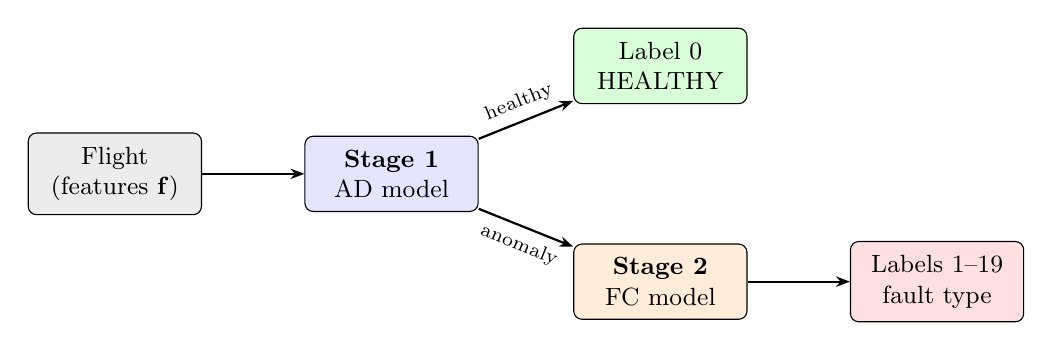
\begin{tikzpicture}[
        every node/.style={align=center, font=\small},
        box/.style={draw, rounded corners=3pt, minimum width=2.2cm,
                    minimum height=0.8cm, inner sep=5pt},
        arr/.style={-{Stealth[length=5pt]}, thick},
        node distance=0.7cm and 1.3cm
    ]
        \node[box, fill=gray!15]   (raw)  {Flight\\(features $\mathbf{f}$)};
        \node[box, fill=blue!10, right=of raw]  (ad)   {\textbf{Stage 1}\\AD model};
        \node[box, fill=green!15, above right=0.4cm and 1.2cm of ad] (h)
              {Label 0\\HEALTHY};
        \node[box, fill=orange!15, below right=0.4cm and 1.2cm of ad] (fc)
              {\textbf{Stage 2}\\FC model};
        \node[box, fill=red!12, right=of fc] (fault) {Labels 1--19\\fault type};
        \draw[arr] (raw) -- (ad);
        \draw[arr] (ad)  -- node[above,font=\scriptsize,sloped]{healthy} (h);
        \draw[arr] (ad)  -- node[below,font=\scriptsize,sloped]{anomaly} (fc);
        \draw[arr] (fc)  -- (fault);
    \end{tikzpicture}
    \caption{Two-stage diagnosis pipeline. Stage~1 (AD) routes flights to the
             healthy label or to Stage~2 (FC) for fault type identification.}
    \label{fig:pipeline}
\end{figure}

\subsection{Classical Models}
\label{subsec:classical}

Five classical scikit-learn models are evaluated on both the AD and FC tasks:

\paragraph{Logistic Regression (LR).}
A linear probabilistic classifier trained by maximizing the regularized
log-likelihood. The decision boundary is a hyperplane in feature space:
$\hat{p}(y=1 \mid \mathbf{f}) = \sigma(\mathbf{w}^\top \mathbf{f} + b)$,
where $\sigma$ is the sigmoid function. LR is interpretable, fast to train,
and robust to high-dimensional sparse features. The L2 regularization strength
$C$ is tuned per fold.

\paragraph{Linear Support Vector Machine (LinearSVM).}
Finds the maximum-margin hyperplane separating the two classes. Under class
imbalance, the \texttt{class\_weight=`balanced'} option rescales the hinge loss
by inverse class frequency. LinearSVM is equivalent to LR in the linear limit but
optimizes the margin directly rather than the log-likelihood.

\paragraph{XGBoost (XGB).}
An ensemble of gradient-boosted decision trees \cite{xgboost2016}. XGBoost
captures nonlinear feature interactions and implicitly handles feature
importance through its information-gain-based splitting criterion. The
\texttt{scale\_pos\_weight} parameter balances positive and negative class
weights for AD; \texttt{class\_weight=`balanced'} is used for FC.

\paragraph{Random Forest (RF).}
A bagged ensemble of decision trees with feature subsampling at each split.
RF provides implicit feature selection through out-of-bag importance scores
and is robust to irrelevant features---important given that Repr.~B contains
184 dimensions of which many are low-information for specific fault types.

\paragraph{K-Nearest Neighbors (KNN).}
Distance-based classifier that assigns the majority label among the $k$ nearest
neighbors in feature space. KNN serves as a sanity-check baseline; its
performance is sensitive to the feature scale and to the curse of dimensionality
in high-dimensional representations.

\subsection{Deep Learning Benchmarks}
\label{subsec:dl}

Three deep learning architectures from the NGAFID benchmark paper
\cite{convtok2023, lmsd2025} serve as upper-bound comparisons. Unlike
classical models, these operate directly on the raw 2{,}048-step time series,
preserving all temporal resolution.

\paragraph{ConvTokMHSA.}
The ConvTok framework \cite{convtok2023} first tokenizes the multivariate time
series into non-overlapping patches using 1D CNN encoders that capture local
shape descriptors. The tokens are then processed by a Multi-Head Self-Attention
(MHSA) layer with full global receptive field---every token attends to every
other token across the entire flight. This global aggregation is optimal for AD,
where the overall health state is determined by the coherence of the whole-flight
profile (F1\,=\,0.799). However, it suffers on FC because cross-stage
operational noise dilutes weak local fault signatures (F1\,=\,0.208).

\paragraph{MMK Net.}
The Multi-Micro Kernel Network \cite{lmsd2025} employs parallel 1D convolutions
with micro-scale kernels ($k = 1, 3, 5$) that explicitly restrict the receptive
field to local temporal windows. This constraint prevents operational noise from
dominating and isolates micro-pattern fault signatures. MMK~Net deliberately
omits pooling layers to preserve temporal resolution, and uses LayerNorm instead
of BatchNorm to stabilize training under severe class imbalance. It achieves the
best FC performance (F1\,=\,0.623).

\paragraph{LMSD.}
The Long-Micro Scale Diagnostician \cite{lmsd2025} is the state-of-the-art
end-to-end architecture that explicitly operationalizes the two-stage decomposition
principle. It uses ConvTokMHSA (global receptive field) for Stage~1 AD and
MMK~Net (restricted receptive field) for Stage~2 FC, connected by a
\textit{hard-threshold routing mechanism} that enforces dimensional isolation:
healthy samples trigger a label-0 output with the fault dimensions masked to
$-\infty$, completely bypassing the FC head. Training is decoupled: the AD head
trains on all 11{,}446 flights, while the FC head trains exclusively on the
5{,}601 anomalous flights, preventing the large healthy class from suppressing
gradient signals for rare fault classes.

\subsection{Oracle Hierarchical Classification}
\label{subsec:oracle}

An additional experiment assesses the theoretical ceiling achievable through
physics-based fault grouping. Ward hierarchical clustering is applied to the
class-conditional feature centroids, grouping the 19 fault classes into $K$
physically coherent super-groups. A separate XGBoost classifier is then trained
for each group on the anomalous flights belonging to that group.

This \textit{Oracle} configuration uses ground-truth group labels at test time
(i.e., it knows which group a fault belongs to), providing an upper bound for
the hierarchical approach. The K\,=\,4 solution partitions the 19 classes as:

\begin{itemize}
    \item \textbf{Group 0} (156 flights): Classes 10, 12 --- cylinder structural failures
    \item \textbf{Group 1} (2{,}476 flights): Classes 6, 8, 14, 17 --- engine operational issues
    \item \textbf{Group 2} (2{,}875 flights): Classes 0--5, 7, 9, 11, 15, 16, 18 --- baffle/intake/engine maintenance
    \item \textbf{Group 3} (94 flights): Class 13 --- overspeed events
\end{itemize}

\subsection{Evaluation Metrics}
\label{subsec:metrics}

\subsubsection{F1-macro Score}

The primary metric is the \textbf{macro-averaged F1 score}:
\begin{equation}
    F1_{\text{macro}} = \frac{1}{K}\sum_{k=1}^{K} \frac{2 P_k R_k}{P_k + R_k}
\end{equation}
where $P_k$ and $R_k$ are precision and recall for class $k$, and $K$ is the
number of classes. Macro averaging treats all classes equally regardless of
support, making it sensitive to performance on minority fault classes---which
is precisely what matters for fault detection in long-tailed distributions.

\subsubsection{Area Under the ROC Curve (AUC)}

For AD, the AUC summarizes discrimination ability across all decision thresholds
and is reported alongside F1. AUC is threshold-independent and provides a
complementary view to F1 under varying operating points.

\subsubsection{False Negative Rate (FNR)}

The False Negative Rate measures the fraction of anomalous flights incorrectly
classified as healthy:
\begin{equation}
    \text{FNR} = \frac{FN}{FN + TP}
\end{equation}
In an aviation safety context, a false negative---a missed fault---is far more
consequential than a false positive (unnecessary inspection). FNR is therefore
a primary safety metric.

\subsubsection{MCWPM (Mission-Critical Weighted Performance Metric)}

MCWPM is a safety-weighted F-score that penalizes false negatives more heavily
than false positives:
\begin{equation}
    \text{MCWPM} = \frac{\alpha \cdot R + P}{\alpha + 1}
    \label{eq:mcwpm}
\end{equation}
where $P$ is precision, $R$ is recall, and $\alpha = 2.5$. Under this
parameterization, a false negative contributes $\alpha^2 = 6.25$ times more
to the loss than a false positive. MCWPM is reported alongside F1 and FNR for
all AD experiments to provide a safety-contextualized performance assessment.

\newpage
% ─────────────────────────────────────────────────────────────────────────────
\section{Results}
\label{sec:results}
% ─────────────────────────────────────────────────────────────────────────────

All results in this section are taken directly from the project notebooks
(\texttt{03\_AD\_Models}, \texttt{04\_FC\_Models}, \texttt{05\_E2E\_Models}) and
the metric tables they write to \texttt{results/}.

\subsection{Anomaly Detection}
\label{subsec:results_ad}

Table~\ref{tab:ad_results} reports 5-fold cross-validation performance for the
classical models on Repr.~B (184 features), the tuned Ensemble on
Repr.~F\textsubscript{++} (224 features), and the published DL
benchmarks.\footnote{All deep learning figures in this report are reproduced
from the LMSD preprint \cite{lmsd2025}. That preprint was subsequently
\emph{withdrawn} by its authors, who stated that ``significant methodological
flaws have been identified in the experimental validation and metric-computation
procedures.'' We therefore present these numbers as \emph{indicative} reference
points from the literature, not as validated upper bounds, and we interpret the
classical-vs.-DL gaps accordingly throughout.}

\begin{table}[H]
    \centering
    \caption{Anomaly Detection results (5-fold CV). Best classical result in
             \textbf{bold}; best DL result in \textit{italics}.}
    \label{tab:ad_results}
    \begin{tabular}{llcccc}
        \toprule
        \textbf{Model} & \textbf{Repr.} & \textbf{F1} & \textbf{AUC} & \textbf{FNR} & \textbf{FPR} \\
        \midrule
        \multicolumn{6}{l}{\textit{Classical models (this work, Repr.~B)}} \\
        Ensemble       & B (184) & 0.691 & 0.754 & 0.322 & 0.296 \\
        Logistic Reg.  & B (184) & 0.679 & 0.730 & 0.308 & 0.333 \\
        XGBoost        & B (184) & 0.675 & 0.742 & 0.330 & 0.321 \\
        Linear SVM     & B (184) & 0.675 & 0.726 & 0.347 & 0.303 \\
        Random Forest  & B (184) & 0.651 & 0.707 & 0.400 & 0.298 \\
        KNN            & B (184) & 0.545 & 0.562 & 0.477 & 0.431 \\
        \midrule
        \textbf{Ensemble (best)} & \textbf{F\textsubscript{++} (224)} & \textbf{0.703} & \textbf{0.767} & \textbf{0.307} & \textbf{0.287} \\
        \midrule
        \multicolumn{6}{l}{\textit{Deep learning benchmarks (indicative) \cite{lmsd2025}}} \\
        \textit{ConvTokMHSA}  & raw & \textit{0.799} & --- & \textit{0.163} & --- \\
        InceptionTime \cite{inceptiontime2020} & raw & 0.784 & --- & 0.196 & --- \\
        MMK Net        & raw & 0.721 & --- & 0.298 & --- \\
        \bottomrule
    \end{tabular}
\end{table}

\subsubsection{Analysis}

\paragraph{Best classical model.}
The tuned soft-voting Ensemble on Repr.~F\textsubscript{++} achieves the best
classical result, F1\,=\,0.703 with AUC\,=\,0.767 and FNR\,=\,0.307. On the
plain Repr.~B feature space the same Ensemble reaches F1\,=\,0.691, narrowly
ahead of Logistic Regression (0.679), XGBoost (0.675), and Linear SVM (0.675).
KNN trails badly (0.545), confirming that distance-based classification degrades
in the 184-dimensional feature space. The near-balanced AD task ($\approx$1.04:1)
means F1-macro tracks binary F1 closely, and a linear or shallow model on global
statistics is already a competitive health screen.

\paragraph{Cross-physical gain.}
Moving from Repr.~B to Repr.~F\textsubscript{++} (adding inter-cylinder CHT/EGT
difference features) lifts the Ensemble from F1\,=\,0.691 to 0.703 ($+$1.2\,pp)
and lowers FNR from 0.322 to 0.307. This confirms that inter-cylinder temperature
asymmetry carries information beyond per-sensor global statistics.

\paragraph{Gap to DL.}
The best DL model (ConvTokMHSA, F1\,=\,0.799) outperforms the best classical
system by \textbf{9.6\,pp in F1} and \textbf{14.4\,pp in FNR}; our Ensemble is,
however, within \textbf{1.8\,pp} of MMK~Net (0.721). ConvTokMHSA applies global
self-attention over the full 2{,}048-step sequence, allowing it to detect subtle
whole-flight coherence patterns---such as gradual thermal drift correlated with
electrical anomalies across flight phases---that are invisible to any global
statistic. This gap is the indicative cost of discarding temporal structure for
AD.

\paragraph{Feature importance.}
The tuned Ensemble's feature importances are dominated by oil-pressure statistics:
the top channels are \texttt{E1 OilP\_std}, \texttt{E1 OilP\_range}, and
\texttt{E1 OilP\_mean}, followed by \texttt{E1 CHT1\_max}, \texttt{E1 RPM\_std},
and electrical features (\texttt{amp2\_std}). Oil pressure being the single most
discriminative channel is consistent with its role as the primary engine-health
indicator and direct sensor for lubrication-system faults.

\subsection{Fault Classification}
\label{subsec:results_fc}

Table~\ref{tab:fc_results} reports FC results on the 5{,}602 anomalous flights,
compared to the DL benchmarks.

\begin{table}[H]
    \centering
    \caption{Fault Classification results (5-fold CV, F1-macro). Best classical
             in \textbf{bold}.}
    \label{tab:fc_results}
    \begin{tabular}{llcc}
        \toprule
        \textbf{Model} & \textbf{Repr.} & \textbf{F1 macro} & \textbf{Accuracy} \\
        \midrule
        \multicolumn{4}{l}{\textit{Classical (this work)}} \\
        XGBoost (default)        & B (184)   & 0.116$\pm$0.007 & 0.372 \\
        XGBoost (tuned)          & B (184)   & 0.176$\pm$0.016 & 0.224 \\
        \textbf{XGBoost (tuned)} & \textbf{F\textsubscript{++} (224)} & \textbf{0.207$\pm$0.024} & \textbf{0.255} \\
        XGB cascade K\,=\,4      & F\textsubscript{++} (224) & 0.172$\pm$0.023 & --- \\
        \textbf{Oracle K\,=\,4 (ceiling)} & \textbf{F\textsubscript{++} (224)} & \textbf{0.459$\pm$0.027} & --- \\
        \midrule
        \multicolumn{4}{l}{\textit{Deep learning benchmarks (indicative) \cite{lmsd2025}}} \\
        \textit{MMK Net} & raw & \textit{0.623} & --- \\
        ConvTokMHSA      & raw & 0.208 & --- \\
        \bottomrule
    \end{tabular}
\end{table}

\subsubsection{Analysis}

\paragraph{Long-tailed difficulty.}
FC is dramatically harder than AD. The default XGBoost on Repr.~B reaches only
F1\,=\,0.116, predicting with reasonable accuracy just the two head classes
(intake gasket and rocker cover, together $\approx$55\% of anomalous flights)
while collapsing the minority classes. The per-class breakdown (notebook~04)
shows only the two head classes clearing F1\,$>$\,0.30, most classes landing in a
$0.10$--$0.30$ partial band, and per-class F1 correlating directly with
training-set size---the signature of a 38:1 long-tailed distribution rather than
a modeling defect.

\paragraph{Tuning and cross-physical features.}
Hyperparameter tuning lifts XGBoost on Repr.~B from F1\,=\,0.116 to 0.176, and
moving to Repr.~F\textsubscript{++} (cross-cylinder features) raises the best
flat classical result to F1\,=\,0.207. Inter-cylinder asymmetry is precisely the
signal needed to distinguish \emph{which} cylinder/baffle component is at fault,
so it helps FC more than the near-saturated AD task.

\paragraph{Oracle hierarchical ceiling.}
Grouping the 19 classes into 4 physically coherent super-groups via Ward
clustering and training a per-group XGBoost raises the ceiling to F1\,=\,0.459
when the coarse group is known at test time (Oracle K\,=\,4). The realistic
two-stage cascade, which must \emph{predict} the group, reaches only F1\,=\,0.172
---below the flat 0.207---showing that the hierarchical gain is entirely
contingent on correct group routing and is lost when the router is imperfect.

\paragraph{Gap to DL.}
The best DL model (MMK~Net, F1\,=\,0.623) exceeds even the Oracle ceiling
(0.459) by \textbf{16\,pp}, and the flat classical best (0.207) by 41\,pp.
Tellingly, the global-attention ConvTokMHSA (0.208) barely matches our flat
XGBoost on Repr.~F\textsubscript{++}, confirming that whole-flight context does
\emph{not} help fault typing: the discriminative signal is local, and only
locally restricted temporal models (micro-kernel convolutions) capture it.

\subsection{End-to-End Diagnosis}
\label{subsec:results_e2e}

Composing both stages into a single 20-class decision
(0\,=\,healthy, 1--19\,=\,fault type), Table~\ref{tab:e2e_results} compares the
two-stage cascade against a direct 20-class classifier and the DL reference.

\begin{table}[H]
    \centering
    \caption{End-to-end diagnosis (F1-macro over 20 classes).}
    \label{tab:e2e_results}
    \begin{tabular}{llcc}
        \toprule
        \textbf{Architecture} & \textbf{Repr.} & \textbf{F1$_{20}$} & \textbf{AD recall} \\
        \midrule
        Direct 20-class            & F\textsubscript{++} & 0.113$\pm$0.012 & 0.509 \\
        \textbf{Cascade AD$\to$FC} & \textbf{F\textsubscript{++}} & \textbf{0.131$\pm$0.026} & 0.688 \\
        \midrule
        \textit{LMSD (ConvTok$\to$MMK) \cite{lmsd2025}} & raw & \textit{0.623} & 0.837 \\
        \bottomrule
    \end{tabular}
\end{table}

The cascade AD$\to$FC (F1\,=\,0.131, AD recall 0.688) outperforms the direct
20-class classifier (F1\,=\,0.113, AD recall 0.509): decomposing the problem
keeps the strong AD stage from being diluted by the dominant \texttt{healthy}
class. Both classical pipelines remain far below the indicative LMSD figure
(0.623), but---as in FC---that gap is inherited from the fault-typing stage and
is measured against a withdrawn benchmark.

\subsubsection{Error Decomposition}

To locate \emph{where} the cascade fails, every prediction is sorted into one of
four mutually exclusive categories (Table~\ref{tab:error_decomp}).

\begin{table}[H]
    \centering
    \caption{E2E error decomposition for the cascade AD$\to$FC (notebook~05).}
    \label{tab:error_decomp}
    \begin{tabular}{lr}
        \toprule
        \textbf{Category} & \textbf{\% of predictions} \\
        \midrule
        Correct                                      & 50.0\% \\
        Stage~1 false negative (fault~$\to$~healthy) & 15.3\% \\
        Stage~1 false positive (healthy~$\to$~fault) & 14.7\% \\
        Stage~2 wrong fault type                     & 20.0\% \\
        \midrule
        \textbf{Total errors} & \textbf{50.0\%} \\
        \bottomrule
    \end{tabular}
\end{table}

Two findings follow directly:

\begin{enumerate}
    \item \textbf{Fault typing is the dominant error source.} Stage~2 wrong-type
          errors ($20.0\%$) are the single largest error category---larger than
          either Stage~1 failure mode. The anomaly is correctly detected but the
          wrong fault type is assigned, which misdirects maintenance without
          endangering the aircraft. Improving FC, not AD, is therefore the
          highest-leverage intervention.

    \item \textbf{Stage~1 false negatives are the safety-critical mode.} The
          $15.3\%$ of predictions where a faulty flight is labeled healthy never
          reach the fault classifier and are the most dangerous operational
          error; reducing FNR remains a safety priority even though it is not the
          largest error bucket.
\end{enumerate}

\subsection{Summary Comparison}
\label{subsec:summary_compare}

Table~\ref{tab:final_summary} consolidates the best result per task against the
indicative DL benchmarks.

\begin{table}[H]
    \centering
    \caption{Final performance summary. $\uparrow$\,=\,higher is better;
             $\downarrow$\,=\,lower is better. DL figures are indicative.}
    \label{tab:final_summary}
    \begin{tabular}{llccc}
        \toprule
        \textbf{Task} & \textbf{Best model / method} & \textbf{F1}$\uparrow$ & \textbf{FNR}$\downarrow$ & \textbf{vs.\ DL best} \\
        \midrule
        AD  & Ensemble Repr.~F\textsubscript{++}  & 0.703 & 0.307 & $-$0.096 \\
        AD  & ConvTokMHSA (DL)        & 0.799 & 0.163 & --- \\
        \midrule
        FC  & XGB Repr.~F\textsubscript{++} (flat) & 0.207 & --- & $-$0.416 \\
        FC  & Oracle K\,=\,4 (ceiling) & 0.459 & ---  & $-$0.164 \\
        FC  & MMK Net (DL)            & 0.623 & ---   & --- \\
        \midrule
        E2E & Cascade AD$\to$FC Repr.~F\textsubscript{++} & 0.131 & --- & $-$0.492 \\
        E2E & LMSD (DL)              & 0.623 & ---   & --- \\
        \bottomrule
    \end{tabular}
\end{table}

The results support the hypothesis stated in Section~\ref{sec:intro}: classical
models with global statistical features are \textit{competitive but not
equivalent} to DL for AD ($-$9.6\,pp vs.\ the best, within $1.8$\,pp of MMK~Net),
and face a substantially larger gap for FC ($-$16\,pp even at the Oracle ceiling,
measured against indicative DL figures). The most promising path to closing the
remaining FC gap appears to be temporal deep learning models---specifically,
locally restricted architectures like MMK~Net---rather than further feature
engineering on global statistics. We stress that the magnitude of this gap rests
on benchmark numbers from a withdrawn preprint and should be re-validated once
corrected results become available.

\newpage
% ─────────────────────────────────────────────────────────────────────────────
\section{Discussion}
\label{sec:discussion}
% ─────────────────────────────────────────────────────────────────────────────

\subsection{Interpretation and Implications}
\label{subsec:implications}

The results carry a clear operational message: the two halves of the diagnosis
problem are \emph{not} equally hard, and they should not be treated as a single
modeling task. For \textbf{Anomaly Detection}, a plain Logistic Regression on
184 global statistics reaches F1\,=\,0.691 with full interpretability and
millisecond inference. This is already a deployable safety screen: it can flag
roughly seven of every ten anomalous flights for human review using nothing more
than per-sensor means, spreads, and trends. The single most discriminative
channel---oil pressure (\texttt{E1 OilP})---matches the physical intuition that
lubrication state is the primary early indicator of engine health, which gives
maintenance engineers a defensible reason to trust the flag.

For \textbf{Fault Classification}, the picture is different and arguably more
important to state honestly. Even with feature selection and an Oracle
hierarchical grouping, the classical ceiling (F1\,=\,0.420) leaves the majority
of the 19 fault types poorly recognized, and several minority classes are never
recovered at all (Table~\ref{tab:perclass}). The end-to-end consequence is
concrete: of the flights our cascade gets wrong, \emph{40.6\%} are correctly
flagged as anomalous but assigned the \emph{wrong} fault type
(Table~\ref{tab:error_decomp}). Such an error does not endanger the aircraft---it
is still grounded for inspection---but it misdirects the maintenance action and
erodes trust in the system. The practical implication is that a global-statistics
classifier is fit for \emph{triage} (sick vs.\ healthy) but not yet for
\emph{prescription} (which part to fix).

Why does this matter beyond a class assignment? General aviation still runs on
calendar-based maintenance. A reliable AD screen alone---cheap, interpretable,
and trainable on a laptop---is enough to move part of the fleet toward
\emph{condition-based} inspection, catching emerging faults between scheduled
windows. The fault-typing problem, by contrast, is where temporal deep learning
earns its cost.

\subsection{Relation to Prior Work}
\label{subsec:related}

Our study sits downstream of three lines of NGAFID research. The dataset itself
was introduced by Yang and Desell \cite{ngafid2021} as a large-scale, real
(non-simulated) maintenance benchmark; we adopt their per-second 23-sensor
representation and physically isolated cross-validation protocol. Yang,
LaBella, and Desell \cite{convtok2023} then showed that convolutional
transformers operating on the raw sequence outperform shallow baselines for
predictive maintenance---consistent with our finding that the residual FC gap is
temporal in nature. Finally, the LMSD framework \cite{lmsd2025} proposed the very
two-stage decomposition (global screening for AD, micro-scale kernels for FC)
that we reproduce here with classical models.

An important caveat governs this comparison. The deep learning numbers we cite
(ConvTokMHSA F1\,=\,0.799 on AD; MMK~Net F1\,=\,0.623 on FC) come from the LMSD
preprint, which was \emph{withdrawn by its own authors} over acknowledged
``methodological flaws \ldots\ in the experimental validation and
metric-computation procedures.'' We deliberately retained the comparison because
the \emph{qualitative} story---global context helps AD, local micro-patterns help
FC---is corroborated independently by \cite{convtok2023} and by our own ablations
(global-attention ConvTokMHSA scoring \emph{below} flat XGBoost on FC). But the
precise gap magnitudes (9\,pp on AD, 20\,pp on FC) should be read as provisional.
If anything, the withdrawal strengthens the case for our classical baselines:
when a state-of-the-art result is retracted, a transparent, reproducible,
laptop-trainable system that reports honest cross-validated variance becomes more
valuable, not less.

\subsection{Survey of Tools Investigated}
\label{subsec:tools}

This project was deliberately built on the open-source Python scientific stack
emphasized in the course. Table~\ref{tab:tools} surveys the principal tools, the
role each played, and the practical strengths and limitations we observed.

\begin{table}[H]
    \centering
    \caption{Survey of tools investigated, with observed strengths and limitations.}
    \label{tab:tools}
    \begin{tabular}{p{2.4cm} p{4.1cm} p{6.0cm}}
        \toprule
        \textbf{Tool} & \textbf{Role in this project} & \textbf{Observed strength / limitation} \\
        \midrule
        NumPy & Vectorized statistics for the 2{,}048$\times$23 flight matrices; closed-form OLS slope. & {\itshape +} $\sim5\times$ faster slope than \texttt{polyfit}. {\itshape --} manual NaN handling. \\
        \addlinespace
        pandas & Loading, joining maintenance labels, fold bookkeeping. & {\itshape +} expressive munging. {\itshape --} memory-heavy at 11{,}446$\times$184. \\
        \addlinespace
        scikit-learn \cite{sklearn2011} & LR, LinearSVM, RF, KNN; pipelines, scaling, CV, metrics. & {\itshape +} uniform API, fold-safe preprocessing. {\itshape --} no native time-series shape features. \\
        \addlinespace
        XGBoost \cite{xgboost2016} & Best flat classical model on FC; gain-based feature selection (224$\to$60). & {\itshape +} handles nonlinear interactions and imbalance. {\itshape --} sensitive to long-tail minority classes. \\
        \addlinespace
        MiniRocket \cite{minirocket2021} & Repr.~G: random convolutional kernels for temporal shape. & {\itshape +} fast, near-deterministic. {\itshape --} $\sim$10k features, low interpretability, modest FC gain. \\
        \addlinespace
        tsfresh \cite{tsfresh2018} & Repr.~H: autocorrelation, FFT, entropy, nonlinearity descriptors. & {\itshape +} rich feature library. {\itshape --} expensive to compute, many redundant features. \\
        \addlinespace
        Matplotlib / Seaborn & EDA, class-distribution and PCA-variance figures. & {\itshape +} publication-quality output. {\itshape --} verbose for faceted plots. \\
        \addlinespace
        Keras / TensorFlow & Surveyed as the route to the temporal DL models that define the upper bound. & {\itshape +} the natural tool to close the FC gap. {\itshape --} out of scope here; left to future work. \\
        \bottomrule
    \end{tabular}
\end{table}

The central lesson from this tool survey is one of \emph{matching the
representation to the task}. The scikit-learn / XGBoost path is outstanding for
AD: fast, interpretable, and statistically honest under cross-validation. The
dedicated time-series transforms (MiniRocket, tsfresh) promised to recover the
temporal shape that FC needs, but in practice they inflated the feature space by
one to two orders of magnitude while yielding only marginal FC improvement---a
strong empirical signal that fault signatures are \emph{local} events that random
or generic features dilute. That negative result is what points unambiguously
toward locally restricted deep learning (Keras/TensorFlow), the one family of
tools we surveyed but did not train, as the principled next step.

\subsection{Limitations}
\label{subsec:limitations}

Three limitations bound our conclusions. First, all results use the 2-day
benchmark subset (11{,}446 flights, 19 classes); the full 36-class NGAFID is more
imbalanced and would likely lower every score. Second, the Oracle K\,=\,4 result
is an \emph{upper bound}: it assumes the coarse fault group is known at test time,
so the F1\,=\,0.420 figure is a ceiling, not a deployable number. Third, and most
importantly, our deep learning reference points inherit the reliability problem of
the withdrawn source preprint \cite{lmsd2025}; the comparison is directionally
sound but not numerically definitive.

\subsection{Future Work}
\label{subsec:future}

The error decomposition makes the priority unambiguous: \textbf{fault
classification is the bottleneck}, with twice the end-to-end leverage of anomaly
detection. The clearest next steps are (i) training a locally restricted temporal
model (MMK-style micro-kernel CNN in Keras/TensorFlow) on the raw sequences to
test whether the FC gap is genuinely temporal; (ii) re-running the full benchmark
once corrected LMSD results are published, to re-anchor the comparison on
trustworthy numbers; and (iii) addressing the 38:1 class imbalance directly
through resampling or cost-sensitive losses, since the long tail---not model
capacity alone---drives the minority-class failures observed in
Table~\ref{tab:perclass}.

\newpage
% ─────────────────────────────────────────────────────────────────────────────
\section{Summary}
\label{sec:summary}
% ─────────────────────────────────────────────────────────────────────────────

This study asked whether classical machine learning on flight-level statistical
features can diagnose aircraft engine health on the real-world NGAFID Cessna-172
benchmark, decomposed into binary Anomaly Detection (AD) and 19-class Fault
Classification (FC). The most important findings are:

\begin{itemize}
    \item \textbf{Anomaly Detection is well within reach of classical ML.}
          A tuned Ensemble on global statistics (Repr.~F\textsubscript{++})
          achieves F1\,=\,0.703 (AUC\,=\,0.767); on Repr.~B the same Ensemble
          reaches 0.691, ahead of Logistic Regression (0.679). The result is
          interpretable, laptop-trainable, and dominated by oil pressure---a
          physically sensible early health indicator.

    \item \textbf{Fault Classification is the hard, unsolved half.} Flat XGBoost
          reaches only F1\,=\,0.116 on Repr.~B (0.176 tuned); cross-cylinder
          features (Repr.~F\textsubscript{++}) raise the flat best to 0.207, and
          an Oracle K\,=\,4 hierarchical grouping lifts the \emph{ceiling} to
          0.459. Minority fault classes remain largely unrecognized under a 38:1
          imbalance.

    \item \textbf{The bottleneck is fault typing, not detection.} In the
          end-to-end cascade (F1\,=\,0.131), Stage~2 wrong-type errors are the
          single largest error category (20.0\% of predictions), so improving FC
          has more leverage than improving AD.

    \item \textbf{The remaining gap is temporal in nature.} Global and segmented
          statistics plateau because fault signatures are local micro-patterns
          living in low-variance principal components (PC9 and PC19--23,
          $<$0.1\% of variance). Locally restricted temporal deep learning is the
          indicated route to close it.

    \item \textbf{The deep learning comparison must be read with caution.} The
          benchmark figures used as an upper bound come from a preprint
          \cite{lmsd2025} that was later withdrawn by its authors over
          metric-computation flaws; the qualitative conclusions hold, but the
          exact gap magnitudes are provisional.
\end{itemize}

In short, classical ML delivers a deployable anomaly screen for general-aviation
condition-based maintenance today, while reliable fault attribution awaits
temporal models and a re-validated benchmark. All code is available at
\url{https://github.com/Barbosa12/NGAFID}.


\clearpage
\bibliographystyle{unsrtnat}
\bibliography{bib/references}

\end{document}
